\chapter{INTRODUCTION\label{chapter:introduction}}
The nature of scientific models is a deep philosophical topic \citep{giere2010explaining}, \citep{morrison2009models}, \citep{frigg2006models}.
For the purposes of this thesis, we will consider a family of abstracted scientific models as assertions about a collection of variables that refer to aspects of the world, along with a set of functional relations between variables that stipulate how the state of one variable is a function of zero or more other variables. We refer to these as {\em executable} models. Executable models specify enough detail such that given values of input variables, the model can calculate the state of all of the other variables of the model. 
This form of %scientific 
model can be represented as a graph, such as that shown in Figure~\ref{fig:example_sci_model}, where variables (ovals) are connected to one another by functions (boxes) that determine how variables influence each other.
As shown in the figure, % scientific 
models like these can be used to study real-world systems by making a claim (potentially directly testable) about how different observed states of the world are causally related: the executable model asserts that states of parent (input) variables will (partially) determine the states of child (output) variables as according to the function between the variables.
Additionally, uncertainty in variables % measured values 
can be represented explicitly by an empirical or estimated distribution over variable values. For example, the empirical distribution over {\tt Total Daily Rainfall} in Fig~\ref{fig:example_sci_model} is used to characterize the uncertainty in the {\tt Water} input variable to the model. 
% Distributions can be imposed over input variables that track the uncertainty present in the values that the input might take.
Using the functions included in the model that describe how variables effect each other, the uncertainty imposed upon the inputs then induces a distribution over output variable of the model: In Fig.~\ref{fig:example_sci_model}, this is seen in the distribution over predicted {\tt Crop Yield} values, which is a direct result of the uncertainty in amount of {\tt Water} present.

\begin{figure}[!htbp]
  \centering
  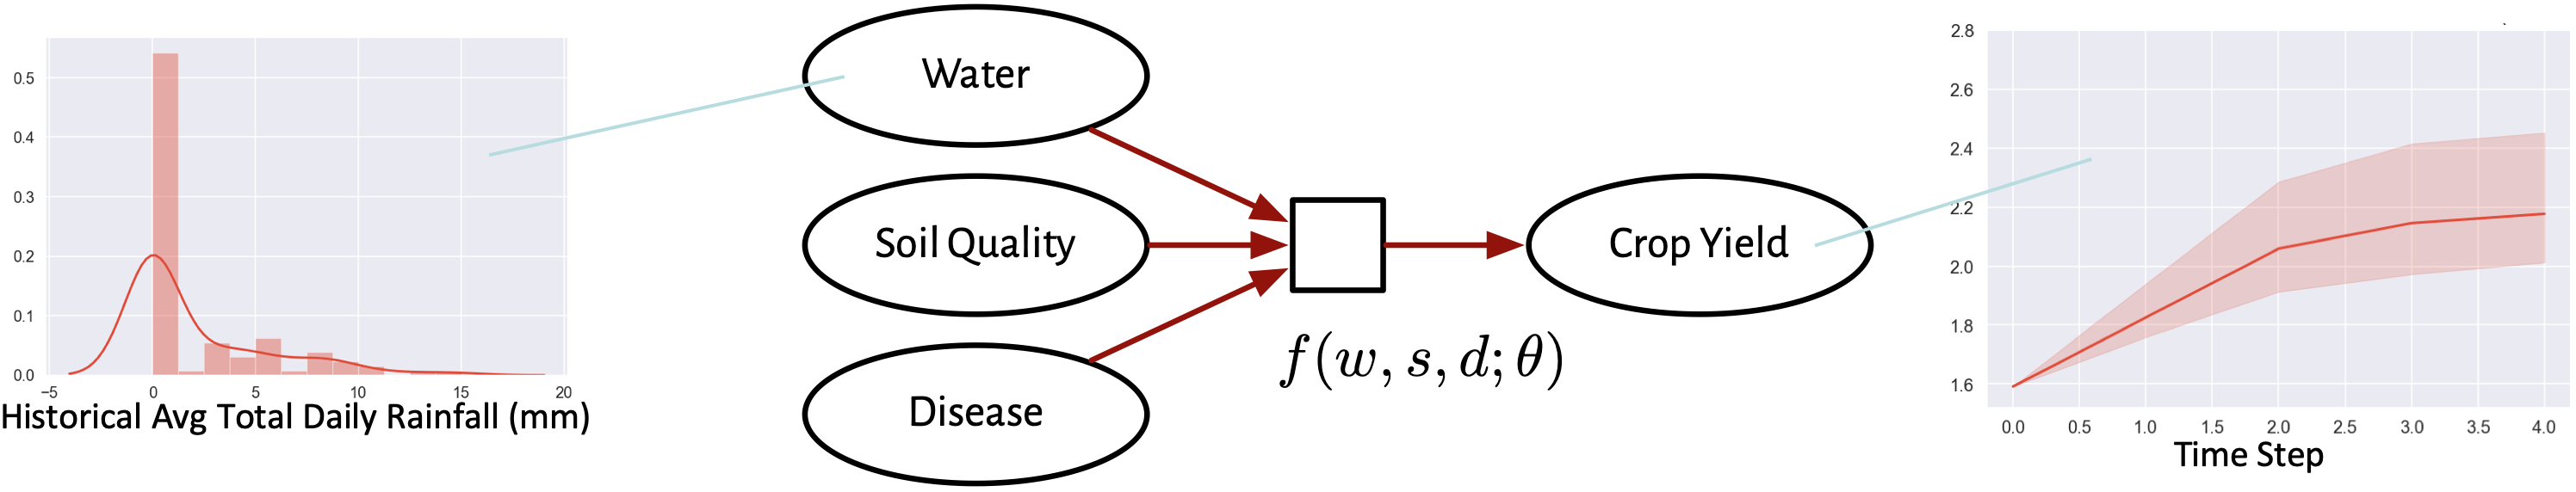
\includegraphics[width=\textwidth]{example_scientific_model}
  \caption[Example of a Scientific Model]{An illustration of an executable model that shows how a distribution over a model input can be used to make predictions about the models output.}
  \label{fig:example_sci_model}
\end{figure}

Translating knowledge about the uncertainty present in the inputs of a scientific model into a statement about the uncertainty of the models output gives domain modelers an incredibly useful tool: the ability to make predictions along with a basis for assessing our confidence in the predictions.
Not only are scientific models able to make predictions, but the structure of models as a functional representation of variables allows those predictions to be interpreted and explained.
Consider the following question that could be posed to a team of domain modelers:
\begin{quote}
\textit{Will South Sudan be able to generate and deliver enough food to its population over the next three years?}
\end{quote}
At its core, this question is asking domain modelers to make a prediction about the state of several real-world variables.
For this example, domain modelers need to be able to make predictions about the expected food production, the expected population size, and the expected security of food transportation networks of South Sudan for the next three years.
The importance of this question also dictates that the predictions proposed by the domain modelers comes with an interpretable explanation that accounts for why the predictions are what they are.
Domain modelers can design a scientific model to answer each of the component questions included in the overall question, where each model will provide an explainable prediction.
This ability to make explainable predictions, such as the ones necessary to answer important questions including the one above, has particularly led to the increasing adoption of executable models by the scientific community for studying complex systems.

\section{Motivation\label{sec:motivation}}
The use of %scientific 
executable models has lead to the development of many supporting tasks that are carried out by \emph{domain modelers}, the scientists who seek to use models in their research studying a specific domain.
In general, science is driven by the repeated process of proposing multiple different, competing models of how observable phenomena may work.
%An example of such a task stems from the fact that for many systems of observable phenomena, multiple competing scientific models of the system exist.
An simple example of such a situation is shown in Figure~\ref{fig:simple_crop_CAG}, which depicts two competing models, each of which seeks to describe how the yield of a particular crop is affected by changes in the amount of rain and soil water absorption rate over time (expressed in \emph{Day}s).

\begin{figure}[!htbp]
  \centering
  \tikz{ % Simple Crop Yield model example
    \tikzstyle{readable}=[rectangle, thick, rounded corners]
    \node[latent, readable] (crop_yield) {$Yield$} ; %
    \node[latent, readable, above=of crop_yield] (total_rain) {$Rain_{total}$} ; %
    \node[latent, readable, above=of total_rain] (rain) {$Rain$} ; %
    \node[obs, readable, above=of rain] (max_rain) {$Rain_{max}$} ; %
    \node[obs, readable, left=of max_rain] (absorption) {$Absorption$} ; %
    \node[obs, readable, right=of max_rain] (consistency) {$Consistency$} ; %
    \node[obs, readable, right=of rain] (day) {$Day$} ; %
    \edge {day, consistency, absorption, max_rain} {rain} ; %
    \edge {rain} {total_rain} ; %
    \path [->] (total_rain) edge  [loop right] (total_rain);
    \edge {total_rain} {crop_yield} ; %

    \plate {loop} {(rain)(day)(total_rain)} {$Day$} ;
  }
  \tikz{ % Different Crop Yield model example
    \tikzstyle{readable}=[rectangle, thick, rounded corners]
    \node[latent, readable] (crop_yield) {$Yield$} ; %
    \node[latent, readable, above=of crop_yield] (total_rain) {$Rain_{total}$} ; %
    \node[latent, readable, above=of total_rain] (rain) {$Rain$} ; %
    \node[obs, readable, above=of rain] (max_rain) {$Rain_{max}$} ; %
    \node[obs, readable, right=of max_rain] (absorption) {$Absorption$} ; %
    \node[obs, readable, left=of rain] (consistency) {$Consistency$} ; %
    \node[obs, readable, left=of total_rain] (sunlight) {$Sunlight$} ; %
    \node[obs, readable, right=of rain] (day) {$Day$} ; %
    \edge {day, absorption, max_rain} {rain} ; %
    \edge {rain, consistency} {total_rain} ; %
    \path [->] (total_rain) edge  [loop right] (total_rain);
    \edge {total_rain, sunlight} {crop_yield} ; %

    \plate {loop} {(rain)(day)(total_rain)} {$Day$} ;
  }
  \caption[Competing Models of Crop Yield]{Two competing scientific models depicting the effects of rain on the yield of a crop over a span of days given a set of input variables (shaded). We see that the two models share many of their inputs but that some inputs may not be shared and the wiring of the inputs to the output variable differs between the two models.}
  \label{fig:simple_crop_CAG}
\end{figure}

We can see that, while the two % scientific 
models shown in the figure share many variables, some variables are not shared between the two models and the directed edges in the two models, representing how one variable’s state is a function of other variable(s) is not identical.
Each of these models makes a different set of claims about how the state of \emph{Yield} is determined by other states of the world.
A critical task of scientific reasoning is to determine which model is a better description of how nature works (or the possibility that neither is a good account).
This is an example of the general task of \textit{model choice}.
The model choice task requires domain modelers to analyze the available competing models of their system of interest and then to select which model best describes the outcomes of experiments or other observations.
Another, closely related task is \emph{model analysis}.
% The process of analyzing the available scientific models of a system is formalized as the task of \emph{model analysis}.
In model analysis, properties of an executable model are studied, such as how sensitive variations in output variables are to changes in input variables. 

% Model analysis involves the analytical study of models to gain information about one or more models that can be used as metrics of model fitness for a given experiment. These metrics of model fitness are especially useful when they are comparative across models such that they can be used to differentiate competing models of the same phenomena. Model analysis also leads to \textit{model comparison} by utilizing of metrics or information about competing models of the same system to compare the fitness of the two models.

\begin{figure}[!htbp]
  \centering
  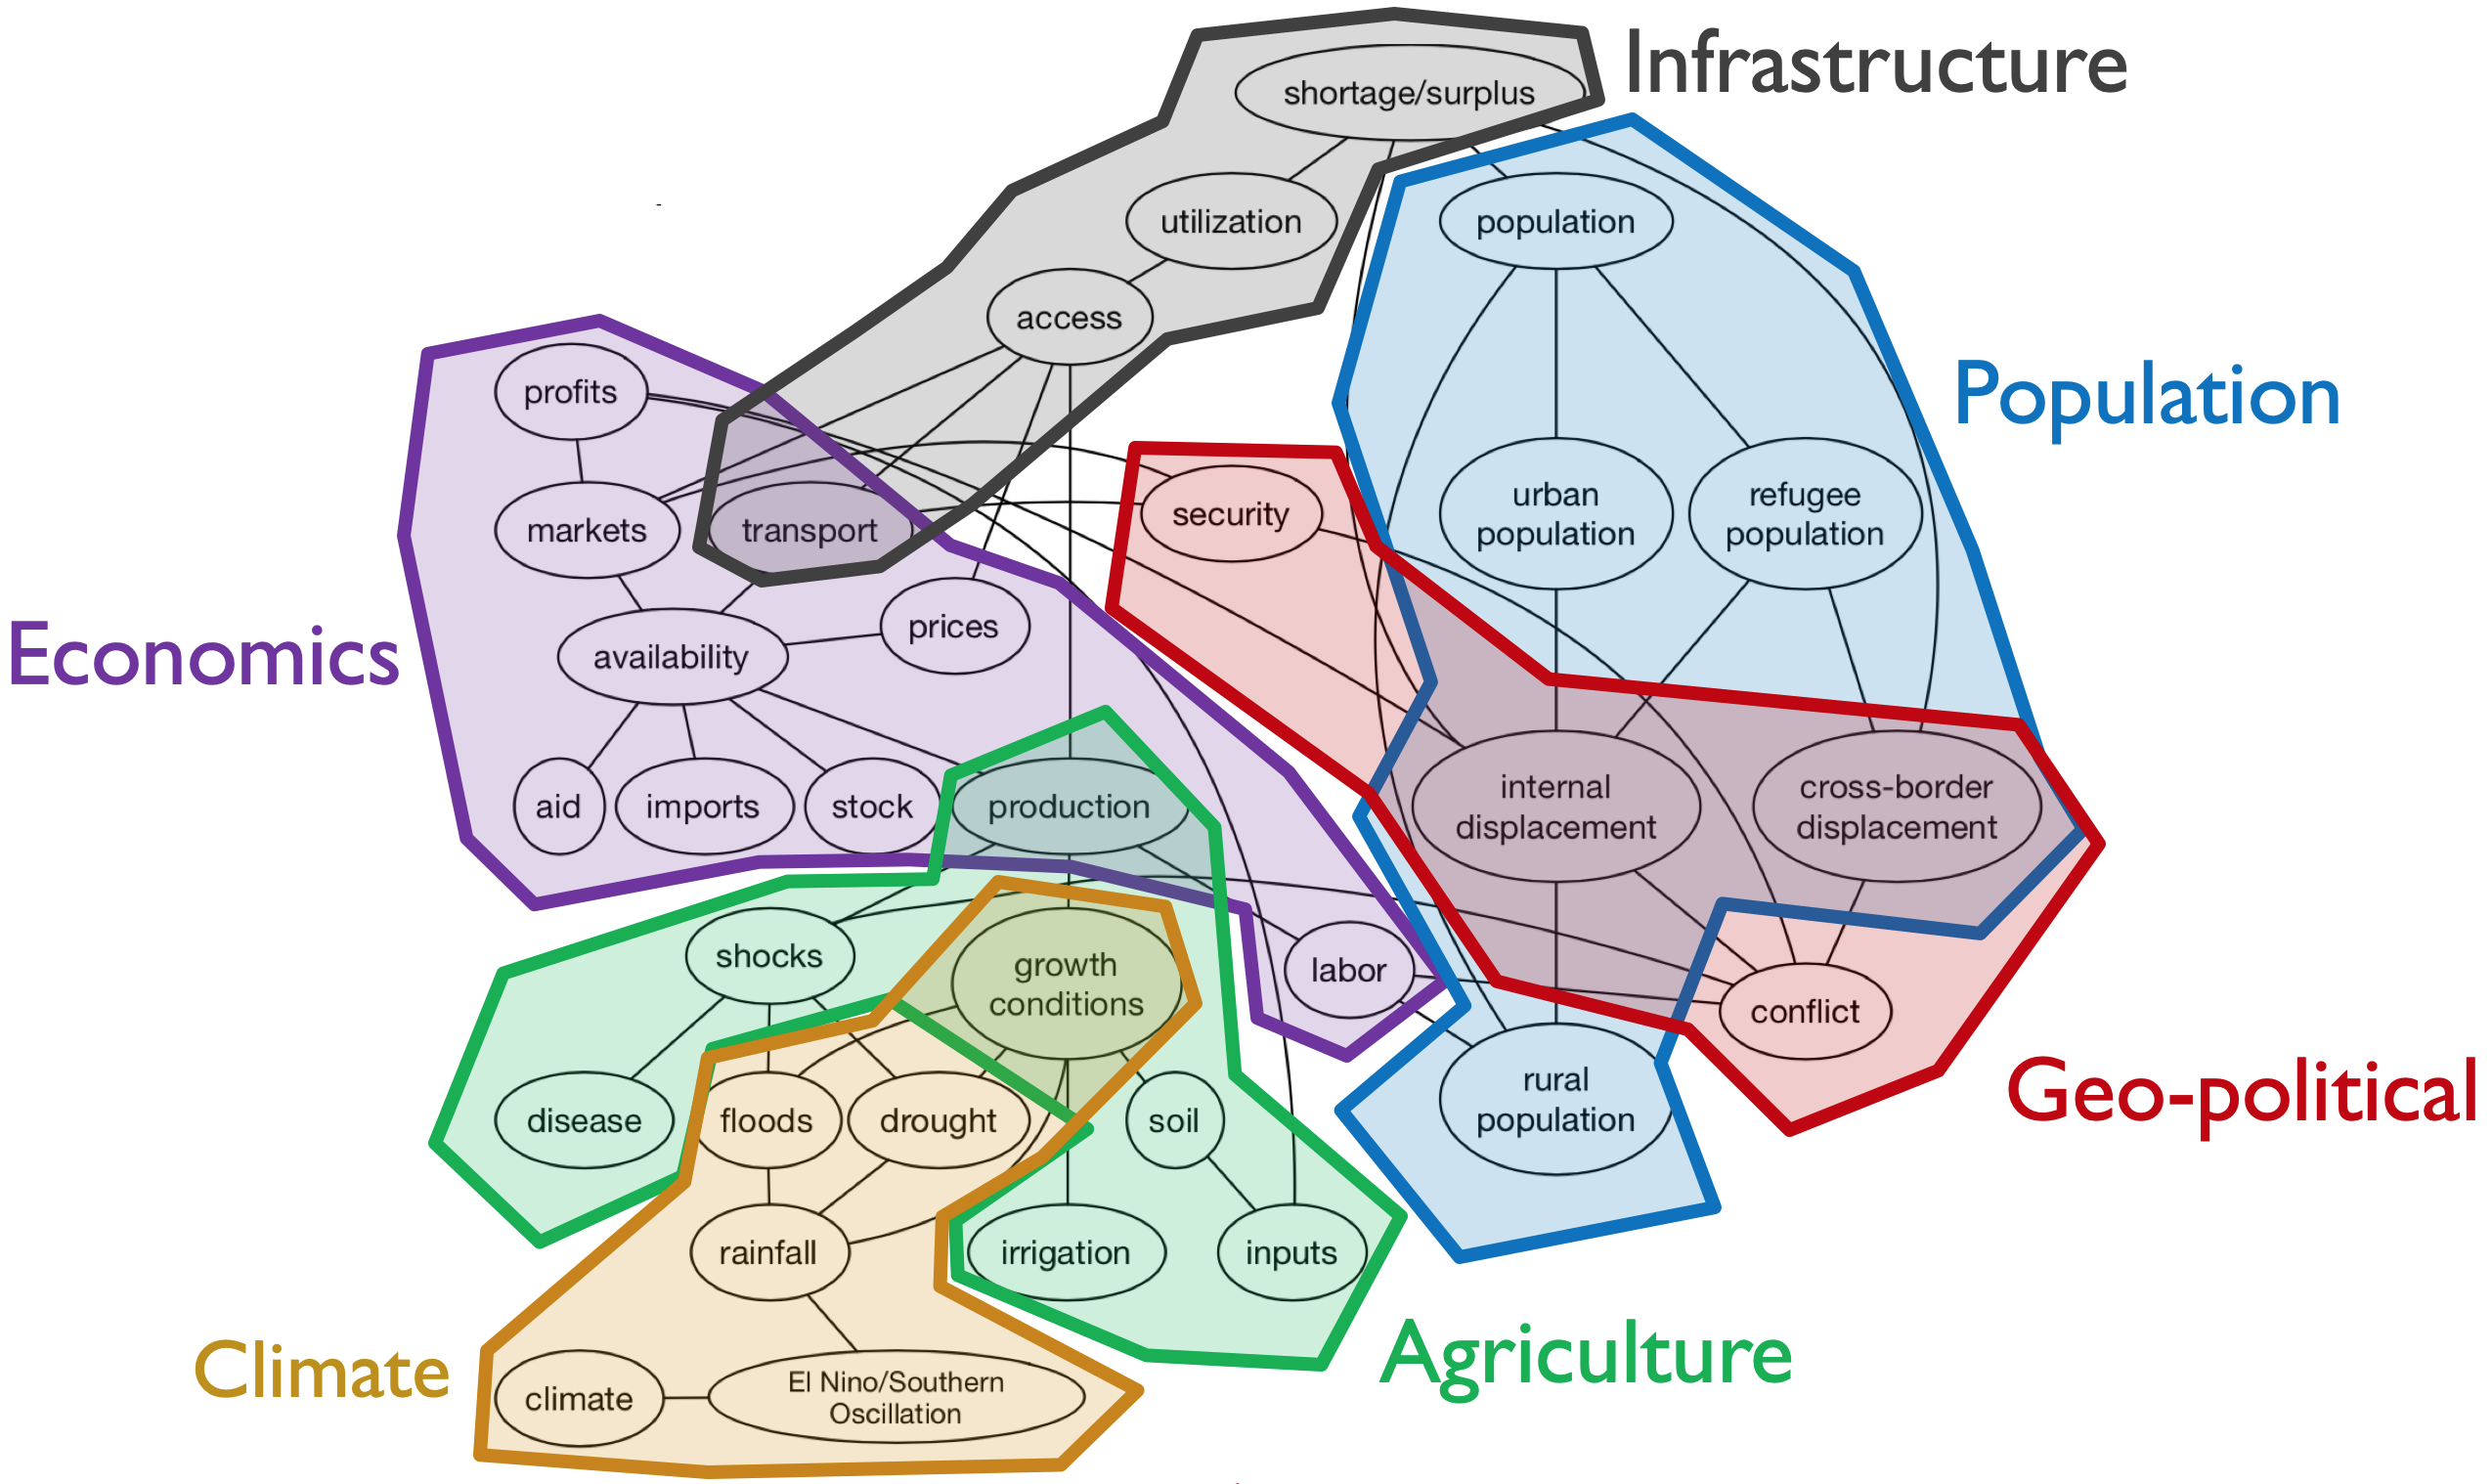
\includegraphics[width=.8\textwidth]{model-composition}
  \caption[Model Composition Web]{An illustration of how multiple scientific models from a diverse array of fields can be combined together to produce a meta-model of a much larger real-world system. In this meta-model each node represents a system that is modeled with a scientific model. Links between nodes correspond to connections between the separate models. Model composition is the process of determining which of these links are appropriate to make.}
  \label{fig:composition_example}
\end{figure}

Similar to how multiple competing models of the same real-world systems exist, there are also models for different aspects of real-world systems that interact with one another.
%Consider the competing models of crop yield shown in Figure~\ref{fig:simple_crop_CAG}. While either of these models can be used to explain the real-world system of crop production, once one is chosen it can be 
Accounting for crop yield as a function of soil, water and disease is just a small part of a much larger set of interacting processes that include the impact of climate on the presence of water and other growing conditions, as well as how the yield impacts local and global economics. A model of crop yield should be composed with other models of related real-world systems to form an aggregate model that now links the interactions between a larger set of world states.
This is the task of \textit{model composition}. 
Figure~\ref{fig:composition_example} presents a ``map'' of the relationships between families of models (colored regions) that describe a number of different aspects of the world that are all involved in predicting and understanding food security.
Models can be composed when links can be identified between models.
These links are commonly in the form of shared model variables, where the output of one model may be the input of another, but more complex linkages can occur as well.
Sometimes a small structure of additional variables must be added in order to compose two models together.
This structure creation is an example of the task of \textit{model augmentation}, which is closely associated with the task of model composition since oftentimes augmentation is required before two models are able to be linked together.

Executable models are generally implemented in a wide range of different programming languages, using a variety of different programming paradigms, and also appear in a context of different conventions for documentation through publications and code comments. Engaging in any of the modeling tasks described above generally requires significant additional labor, such as defining a common model interface that allows for linking of variables, adapting model analysis techniques to specific code bases, or additional coding in a specific code base in order to implement model augmentations. These tasks also require direct involvement of a number of different kinds of expertise, including the domain modelers, model analysts, decision makers, and software engineers.

In this thesis, I propose a framework to help automate and augment significant portions of this process, in order to reduce the additional labor required to bring models together into a common representation.
%Obtaining such a collection of well-represented models requires \textit{source curation} to discover materials that can be used to construct the models and a process of 
In particular, I propose a set of methods for \textit{model extraction and assembly} that can transform raw data from the source code into uniformly represented executable models.
%Improving methods of source curation, model extraction, and assembly improves the access of domain modelers to high quality models that can be used for the other tasks previously mentioned that promote better results when using models.
%Source curation is a challenging and important task for this process; however, it is beyond the scope of this thesis.
%For this thesis we assume that we already have access to the curated data needed and focus on addressing the task of model extraction and assembly.

%Traditionally, manual methods of extraction and assembly have been used by domain modelers to construct the models they need for their studies.
%However, the manual methods of model extraction and assembly do not scale well as the amount of material available to use for model extraction increases.
%In order to deal with the demands for scale in model extraction and assembly, automated methods must be developed that contain the components necessary to extract information about models from the sources where the information is likely to be present and then assemble that information into uniformly represented models that are executable.
%In the information age many model descriptions now exist as software.
%Software implementations of models serve as skeletons that have a high degree guarantee of executability and can be manipulated such that two different software implementations of competing models can be transformed into a uniform representation.
%Adding information from sources such as published texts and documentation associated with the source code allows the uniform, executable skeletons to become models that are ready for use when conducting model analysis, comparison, choice, augmentation, and composition.

\section{Contributions\label{sec:contributions}}
The work presented in this thesis is a component of the larger AutoMATES\footnote{\url{https://ml4ai.github.io/automates/}} (Automated Model Assembly from Text, Equations, and Software) project \citep{pyarelal2019} that is currently under way in the UofA School of Information ML4AI lab.
As the name suggests, the goal of the AutoMATES project is to assemble models from source code and documentation containing definitions of modeling domain concepts and equations that describe the relationships between variables.
To accomplish this goal, the AutoMATES project has three information extraction modules, focused on extracting information about models from the sources mentioned in the AutoMATES title.
The three extraction modules are the Text Reading (TR) module, which extracts information about models from publications and other source texts, the Equation Reading (ER) module, which extracts information from pictures of equations associated with models found in publications, and the Program Analysis (PA) module, which extracts the functional wiring among variables to represent the computation expressed in source code as a dataflow model.

In this thesis, I present my contribution to the AutoMATES project, the \emph{Unified Model Assembly Framework} (UMAF).
As a component of the AutoMATES project, this framework plays the role of automatic assembly of models given the information extracted from the TR, ER, and PA modules.
UMAF integrates source code, text and equation information into a unified representation of a scientific model that will be executable, comparable, and composable.
Combining these capabilities into a single framework provides a facility for domain-expert model developers and analysts to now analyze and compare models within a uniform framework, greatly simplifying model analysis tasks that to-date have required enormous manual effort.

UMAF does not take the human out of the loop: domain expertise and human guidance are still needed to identify variable value ranges of interest to a modeling application, as well as supplement mistakes of omission and commission that may be made during variable grounding.
Ongoing and future development is also required to scale the methods to effectively handle larger model code bases.
UMAF is, to our knowledge, the first general approach to automating model extraction and assembly from source code to support model analysis, comparison, choice, and composition.
We also believe these tools provide a basis for a new kind of model curation and debugging, allowing one to compare changes within evolving code bases but from a modeling domain-semantics perspective; however, exploring use of UMAF for this purpose will be the subject of future work.

\section{Roadmap\label{sec:roadmap}}
This thesis is organized to present how UMAF is able to assemble models from information extraction from source code, text and equations, and then to show how to models created by UMAF can be used to aid modelers in analysis, model choice, and model composition.
During the course of this thesis I will use two models from the Decision Support System for Agrotechnology Transfer (DSSAT)\footnote{\url{https://dssat.net/}} software system \citep{DSSAT} to illustrate the capabilities of UMAF and the associated analysis methods outlined in Section~\ref{sec:contributions}.
The source code used in this study is aimed at modeling the natural phenomena of Potential Evapo-Transpiration (PET).
The specific models I use are the Priestly-Taylor model of Potential Evapo-Transpiration (PETPT) and the ASCE model of Potential Evapo-Transpiration (PETASCE).
Chapter~\ref{chapter:related_work} reviews previous work that has been done in the areas of scientific model extraction, assembly, analysis, comparison, and composition.
Chapter~\ref{chapter:umaf} introduces the algorithms used to assemble models from source code into a form that is both executable and comparable across competing models by utilizing information from source texts to ground variables present in the models.
Finally, Chapter~\ref{chapter:conc_and_future} concludes with a discussion of the results and implications of UMAF and will introduce possible extensions for continuing this research.
